\chapter{Results and Discussion}
\label{ch:4}
\noindent

\section{Computation Times of Fragmentation Expansion}

Computation times present a significant bottleneck for this approach. 
The \texttt{mod} framework, while powerful in generating comprehensive reaction networks, prioritizes flexibility and completeness over computational efficiency. 
Combined with the rapid growth in the number of possible fragments and parent molecules, runtime becomes prohibitive as the number of fragmentation rules increases.
Since only a subset of known rules were applied in this study, computation times per molecule will rise substantially as additional rules are incorporated, making further optimization necessary to ensure the feasibility of this approach at scale.

\subsection{Visualization of Computation Times}

A regression analysis was performed to model the relationship between molecular complexity and computation time. 

Here, molecular complexity refers to Boettcher's complexity measure \cite{Boettcher2016}, which summarizes structural intricacy from the molecular graph. It provides a single scalar descriptor that allows molecules of different sizes and connectivities to be compared on a common scale. In this analysis, it is used as a
proxy for fragmentation difficulty, although runtime is still influenced by additional factors such as the specific structure of the molecule and the available fragmentation pathways.

The analysis assumes:
\begin{itemize}[noitemsep,topsep=0pt]
    %\item Linearity of the relationship
    \item Homoscedasticity of residuals
    \item Independence of residual observations
    \item Normality of residual distribution
\end{itemize}

In Figure \ref{fig:mod-time-regres}, the regression results are visualized, showing a positive correlation between molecular complexity and computation time, but also show a large variance in computation times for molecules of similar complexity.
Note that the threshold of 40 seconds was chosen arbitrarily to exclude trivial expansions.

\begin{figure}[ht]
    \centering
    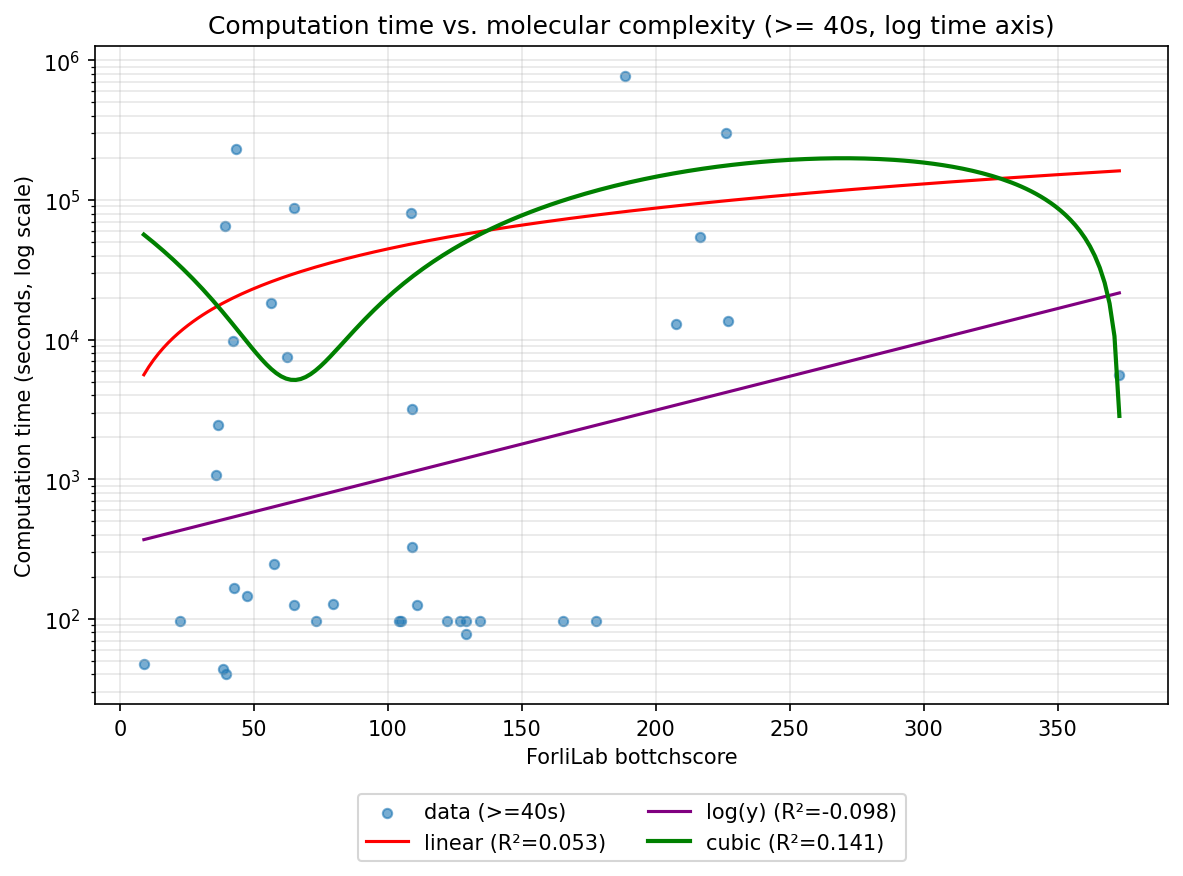
\includegraphics[width=0.8\linewidth]{../shared/figures/time_vs_complexity_logy_over40.png}
    \caption[Fragmentation Computation Times]{
        Regression of Computation time, excluding molecules that had trivial expansions (time $< 40$s).
        The plot shows a positive correlation between molecular complexity and computation time, but also a large variance in computation times for molecules of similar complexity.
        }
    \label{fig:mod-time-regres}
\end{figure}

So while there is a general trend of increasing computation time with molecular complexity, the large variance suggests that other factors, such as specific structural features or the particular fragmentation pathways available, also play a significant role in determining computation time. This highlights the need for further optimization.

\section{Evaluation of Structure--Spectrum Translation}

The evaluation must control for one confound above all others: the precursor (parent) mass.
Because a candidate whose mass matches the query's implied precursor mass is already a strong match, any retrieval score that is not held against a mass baseline can look successful while doing little more than mass filtering.
An earlier version of this pipeline showed the danger directly.
Its free-form spectrum decoder collapsed onto the dataset-mean spectrum --- predicting essentially the same intensity vector regardless of the input molecule --- yet a reranking stage built on top of it still appeared to improve retrieval substantially.
On inspection, that apparent gain was almost entirely a precursor-mass consistency filter: replacing the learned forward spectrum with a constant mean spectrum, or even an all-ones vector, while keeping the mass mask reproduced the same reranking benefit, so the learned spectral shape itself contributed little.

Two changes address this.
First, the fragment-grounded decoder (\Cref{sec:forward-model}) makes each predicted spectrum an explicit function of the molecule's fragment set, so it can no longer collapse to an input-independent spectrum and its peaks land at physically realizable fragment masses by construction.
Second, retrieval is reported under a \emph{mass-controlled} protocol: within a fixed window around the query's true mass, the learned encoder retrieval $\cos(z_{\mathrm{spec}}, z_{\mathrm{mol}})$ is compared against the analytic random-chance baseline for a pool of that size.
Only a result that beats chance \emph{inside} the window counts as learned structural signal, because within a narrow mass window the mass is approximately constant and can no longer explain the ranking.

\subsection{The Forward Model Is Molecule-Specific}
\label{sec:molecule-specific}

With the fragment-grounded decoder, forward prediction is no longer input-invariant.
Averaged over the evaluation molecules, the mean cosine similarity between a predicted spectrum and the mean predicted spectrum is \ph{X.XX}, compared with $\approx 0.999$ for the earlier free-form decoder; predictions therefore vary with the input rather than reproducing a single average spectrum.
For a representative molecule such as benzene, the predicted peaks fall at fragment masses \ph{[m/z list]} that correspond to genuine fragments of the structure rather than at arbitrary bins.
The forward branch thus produces molecule-specific spectra whose support is chemically meaningful, which is the precondition for any use of the forward model in retrieval.

\subsection{Mass-Controlled Retrieval}

The headline evaluation is spectrum-to-structure retrieval assessed against mass.
\Cref{fig:mass-controlled} reports, for held-out test molecules, the learned within-window MRR next to the analytic random-chance MRR for two mass windows.
Within $\pm 5$\,Da the learned retrieval reaches an MRR of \ph{X.XXX} against a chance level of \ph{X.XXX}, a margin of \ph{+X.XXX}; within $\pm 20$\,Da it reaches \ph{X.XXX} against \ph{X.XXX}, a margin of \ph{+X.XXX}.
Because these molecules were seen neither during training nor during model selection, the positive margins indicate that the model recovers structural information that generalizes beyond precursor mass --- the signal that the earlier, collapsed pipeline lacked.

\begin{figure}[H]
    \centering
    \figorpending{width=0.8\linewidth}{../shared/figures/mass_controlled_mrr.pdf}
    \caption[Mass-controlled retrieval: learned vs.\ chance]{
        Spectrum-to-structure retrieval on held-out test molecules, controlled for precursor mass.
        For each mass window ($\pm 5$ and $\pm 20$\,Da around the query's true mass), the learned encoder retrieval MRR is shown next to the analytic random-chance MRR for a pool of the same size.
        A bar standing above its chance reference indicates structural signal that mass alone cannot explain, since mass is approximately constant inside the window.
        This is the decisive test motivated by the forward-collapse analysis: the earlier pipeline's apparent retrieval quality vanished once mass was controlled for, whereas the repaired model retains a positive margin over chance.
    }
    \label{fig:mass-controlled}
\end{figure}

\subsection{Why Raw Retrieval Scores Are Not the Right Axis}
\label{sec:raw-scores}

It is instructive to see how completely mass dominates the uncontrolled metrics, since this is what motivates the mass-controlled protocol.
On the full retrieval gallery, ranking candidates purely by agreement with the query's parent mass is already close to a solution: an oracle ranking by $|\Delta\mathrm{mass}|$ to the true mass reaches an MRR of \ph{X.XX}, and even a spectrum-only mass baseline --- ranking by the mass implied by the query's heaviest peak --- reaches \ph{X.XX}.
Against baselines this strong, the raw learned MRR over the full gallery (\ph{X.XX}) sits at the mass floor and is not, on its own, evidence of learned chemistry.
The full-gallery ablation figures below, comparing the full model against no-fragments, no-derivation-graph, and no-reranking variants, are therefore reported as diagnostics of the pipeline's behaviour rather than as the headline result.

\begin{figure}[H]
    \centering
    \figorpending{width=0.8\linewidth}{../shared/figures/cosine_mrr.pdf}
    \caption[Cosine similarity and MRR for ablation variants]{
        Ablation of three pipeline components (fragments, derivation graph, and reranker) against the full model.
        Cosine similarity measures how similar the query is to the correct target, averaged over all queries; MRR is the mean reciprocal rank of the ground-truth target. 
        Error bars show $95\%$ bootstrap confidence intervals (5000 query resamples). 
        Brackets indicate pairwise p-values from paired randomization tests 
        %on per-query differences (10,000 sign flips), 
        computed separately for each metric. 
        For \emph{cosine similarity}, all variants are nearly identical (\ph{$\approx 0.XX$}) and no pairwise difference is statistically significant, so forward reconstruction is insensitive to the ablations.
        For \emph{MRR}, removing reranking lowers the full-gallery score from \ph{X.XX} to \ph{X.XX} (Full vs.\ no-reranking, $p \approx$~\ph{0.0XX}),
        whereas the fragment and derivation-graph ablations do not differ significantly from the full model.
        As discussed in the text, this full-gallery MRR is dominated by precursor mass, so the reranking effect shown here reflects mass-consistency filtering rather than learned spectral shape.
        }
    \label{fig:cosine-mrr}
\end{figure}

On the forward task, all evaluated variants achieve very similar cosine similarity values.
The full model reaches a mean cosine similarity of \ph{X.XX}, while the no-fragments and no-derivation-graph ablations achieve \ph{X.XX} and \ph{X.XX}, respectively (\Cref{fig:cosine-mrr}).
Unlike in the collapsed pipeline --- where a high cosine was an artefact of every prediction approaching the mean spectrum --- these values now reflect genuine reconstructions; but their near-equality across ablations suggests that the molecular encoder already captures most of the forward-predictive signal, with the fragment branch adding little on this particular metric.

For the full model, Recall@1 is \ph{X.XX}, Recall@5 is \ph{X.XX}, Recall@10 is \ph{X.XX}, and Recall@20 is \ph{X.XX}, with a mean reciprocal rank (MRR) of \ph{X.XX} (\Cref{fig:recall-at-k}).
Read on their own these values resemble a usable candidate-narrowing system, but for the reason established above (\Cref{sec:raw-scores}) they largely reflect precursor-mass agreement; \Cref{fig:mass-controlled} isolates the genuinely learned component.

\begin{figure}[H]
    \centering
    \figorpending{width=0.8\linewidth}{../shared/figures/recall_at_k.pdf}
    \caption[Recall@k for ablation variants]{
        Recall@k for $k = 1, \ldots, 20$ across the full retrieval model and three ablated variants. 
        Shaded bands show 95\% bootstrap confidence intervals over queries. 
        The full model and the \texttt{no fragments}~/~\texttt{no derivation graph} variants cluster together across the full $k$ range, while the \texttt{no reranking} variant trails the others at every $k$, with the largest gap at small $k$ and gradual closure toward $k = 20$.
    }
    \label{fig:recall-at-k}
\end{figure}

On the full gallery, removing reranking leaves the forward cosine similarity unchanged, as expected, but lowers retrieval quality: Recall@5 drops from \ph{X.XX} to \ph{X.XX},
Recall@10 from \ph{X.XX} to \ph{X.XX}, Recall@20 from \ph{X.XX} to \ph{X.XX}, and MRR from \ph{X.XX} to \ph{X.XX}.
Taken at face value this looks like a large benefit from forward-model rescoring, but it is the mass-consistency filtering identified above (\Cref{sec:raw-scores}): the same gain is reproduced by keeping only the precursor-mass mask, so it is not evidence that the learned forward spectral shape drives retrieval.

The fragment-related ablations remain inconclusive on the full-gallery metrics.
Differences between the full model and the no-fragments and no-derivation-graph variants are small and, on query-level paired tests, not statistically convincing, so the full-gallery view does not by itself establish a benefit from the fragment branch.
What the fragment branch does contribute unambiguously is the forward decoder's molecule-specificity (\Cref{sec:molecule-specific}), the property the mass-controlled retrieval result relies on.

These conclusions should be interpreted cautiously.
The held-out test set contains only \ph{XX} queries, so recall values change in coarse increments and differences between variants often reflect only one or two queries.
Model selection was performed on the validation split, so the validation margins over chance are optimistic and the held-out test scorecard of \Cref{fig:mass-controlled} is the figure to trust; the numbers reported here come from a single training run and should be read as a proof of concept rather than a benchmarked result.

Overall, the results show that the proposed bidirectional framework is functional and, once the forward decoder is grounded on fragments, that spectrum-to-structure retrieval carries structural signal beyond precursor mass on held-out molecules.
The decisive evidence is the mass-controlled comparison rather than any raw retrieval score, because the uncontrolled metrics --- including the apparent benefit of reranking --- are dominated by mass consistency.
The main contribution of the present work is therefore twofold: a fragment-augmented bidirectional framework whose forward model is molecule-specific by construction, and a mass-controlled evaluation that separates genuinely learned structural discrimination from mass filtering.
Together these provide a concrete and honestly measured basis for future work aimed at improving the informativeness and integration of fragment-level intermediate representations.

%\section{Forward Model Evaluation}
%\subsection{Spectral Similarity and Fragment Prediction}

%\section{Backward Model Evaluation}
%\subsection{Structure Reconstruction and Validity}
%\subsection{Reward Convergence and Exploration Efficiency}

%\section{Comparison with Baseline Models}
%CFM-ID, 
%
%MSNovelist (https://doi.org/10.1038/s41592-022-01486-3), 
%
%MassGenie (https://doi.org/10.3390/biom11121793) ...


\section{Challenges}
The thesis is shaped by several interconnected challenges. 

\textbf{First}, fragmentation must be represented in a way that is simultaneously chemically meaningful and useful for machine learning. 
\textbf{Second}, explicit fragment generation leads to a \emph{combinatorial explosion} of candidate structures and limits the practical scale of the approach. 
\textbf{Third}, the absence of unique \emph{ground-truth fragmentation graphs} makes fragment-level supervision inherently \emph{ambiguous}.
\textbf{Fourth}, bidirectional learning introduces \emph{competing objectives}, since forward spectrum reconstruction and backward structure retrieval do not necessarily favor the same latent representation. 
Finally and \textbf{fifth}, the empirical contribution of fragment-aware intermediate representations remains difficult to establish conclusively, especially under \emph{small-sample} conditions and in the presence of strong baseline signals from the molecular encoder alone.


%\section{potential improvements}
%speed up graph transformation, especially predicates
%trivial, scoping: use one class of molecules, a diverse set of molecules is naturally more difficult to model.